\documentclass[11pt]{beamer}
\usepackage[utf8]{inputenc}
\usepackage[T1]{fontenc}
%\usepackage{natbib}
\usetheme{Pittsburgh}
\usepackage{verbatim} 
\usepackage[english]{babel}
\usepackage{epstopdf}
%\titlegraphic{%\vspace*{1cm}
%	\includegraphics[width=2.5cm]{logo_udelar}
	%\hspace*{1cm}~%
%		\includegraphics[width=3.5cm]{logo_FCEA.png}
%}
\setbeamertemplate{navigation symbols}{}
%\setbeamertemplate{footline}[frame number]
\AtBeginSection{ 
	\begin{frame}
		\frametitle{Index}
			\tableofcontents[currentsection]
	\end{frame}
}
\begin{document}
	\title{Modelos dinámicos y computacionales en Economía}
	\subtitle{Modelos Basados en Agentes: Difusión de información}
	%\logo{}
	\institute{Licenciatura en Economía, FCEA, UDELAR}
	\date{28 de noviembre de 2024}

	%\subject{}
	%\setbeamercovered{transparent}
	%\setbeamertemplate{navigation symbols}{}
	\frame[plain]{
	\begin{figure}
	\centering
	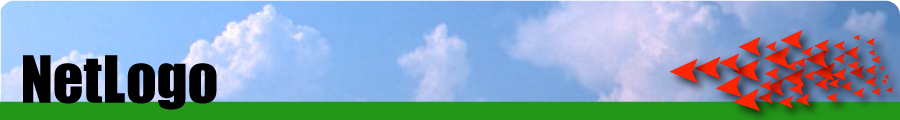
\includegraphics[width=0.7\linewidth]{figuras/netlogo-title-wide-60}
	%		\caption{}
	\label{fig:netlogo-title-wide-60}
\end{figure}	
		\vspace{-1cm}
\maketitle
}
%\setbeamertemplate{background}{\includegraphics[width=2 cm]{logo_FCEA.png}}



\begin{frame}
	\frametitle{Difusión de información}
	¿Cómo modelar transmisión de información?
	\begin{itemize}
		\item<2-> ABM
		\item<3-> Grafos (redes sociales)
	\end{itemize}
	\vspace{2mm}
	Desde distintas ramas de la ciencia se ha estudiado la manera en la cual se difunde la información en las redes sociales.\\
	Dos modelos fundamentales se han propuesto:
	\begin{itemize}
		\item Threshold models of collective behavior (Granovetter, 1978)
		\item Independent Cascade Model (Goldenberg et al., 2001)
	\end{itemize}
\end{frame}

\begin{frame}
	\frametitle{Threshold models of collective behavior}
	\framesubtitle{Granovetter - 1978}
	Propone un modelo aplicable para diversos procesos: segregación residencial, difusión de innovación, huelgas, migración, rumores, enfermedades, votación, etc.
	\begin{itemize}
		\item El punto de partida son las preferencias. A partir de ellas se estudia su agregación.
		\item Individuos racionales
		\footnote{\scriptsize Contrario a los primeros trabajos de la psicología social de la acción colectiva donde se postulaba que acúuan instintiva e irracionalmente (La razón populista - Ernesto Laclau).} y heterogéneos.
		\item Decisiones binarias: paro/no paro, me mudo/no me mudo, voto A/voto B.
		\item Cada agente comienza en la categoría \textit{inactiva}.
	\end{itemize}
	\vspace{3mm}
	¿Cómo simulamos una decisión?
	\begin{itemize}
		\item<2-> Mediante un UMBRAL
	\end{itemize}
\end{frame}

\begin{frame}
	\frametitle{Threshold models of collective behavior}
	\framesubtitle{Umbral de decisión}
	\begin{itemize}
		\item A cada agente se le asigna un umbral aleatoriamente en el intervalo $[0,1]$ (distribución uniforme y normal).
		\item La probabilidad de activación depende de:
		\begin{enumerate}
			\item Lo que hacen los de su comunidad/vecindad.
			\item La influencia de una persona cualquiera sobre el comportamiento de uno (amigo o desconocido).
		\end{enumerate}
		\item Cada vecino tiene un \textit{peso} para representar su influencia.
		\item Una vez que el agente se \textit{activa}, no cambia su estado.
	\end{itemize}
\end{frame}

\begin{frame}
	\frametitle{\normalsize Talk of the Network: A complex systems look at the underlying process of word-of-mouth}
	\framesubtitle{Independent Cascade Model (Goldenberg et al., 2001)}
	\begin{itemize}
			\item La información en la red se difunde a través del \textit{boca a boca}.
			\item Estudian la importancia de la comunicación interpersonal de los vinculos fuertes y débiles (amigos y desconocidos).
			\item Dos estados: activo (nodos que toman en cuenta la información) e inactivo (nodos no influenciados por la información).
			\item Los agentes se pueden informar de 3 formas:
			\begin{itemize}
				\item Contacto con amigo (strong tie)
				\item Contacto con desconocido (weak tie)
				\item Publicidad (con probabilidad $\alpha$)
			\end{itemize}
			\item Cada agente pertenece a una red personal y se conecta con una cantidad finita de desconocidos; el proceso termina cuando se terminan las posibilidades de transmitir información.
	\end{itemize}
\end{frame}

\begin{frame}
	\frametitle{Independent Cascade Model (Goldenberg et al., 2001)}
	\framesubtitle{Funcionamiento del modelo}
	\begin{enumerate}
		\item Todos los agentes empiezan desinformados.
		\item Solo a través de la publicidad se pueden informar: si $U<p(t)_i \Rightarrow$ informado.
		\item Comienza el \textit{boca a boca}: se realizan las probabilidades de activación y el número $U$.
		\item Se repite el paso 3 hasta que el 95\% del total estén informados.
	\end{enumerate}
	\vspace{5mm}
	$$p(t) = (1-(1-\alpha)(1-\beta_w)^j \;(1-\beta_s)^m) \hspace{2mm}
	\footnote{ Donde $\alpha< \beta_w< \beta_s$} $$
	Se simuló el modelo para distintas combinaciones de $\alpha, \beta_w, \beta_s$, tamaño de red personal y número de desconocidos. 
\end{frame}

\begin{frame}
	\frametitle{Independent Cascade Model}
	\framesubtitle{Resultados}
	De las simulaciones extraen datos relevantes para hacer análisis estadístico (regresiones) en distintos momentos (\textit{early informed, middle informed, late informed}).
	\begin{itemize}
		\item La influencia de los contactos débiles en la velocidad de transmisión de información es al menos tan importante como la de los contactos fuertes (\textit{the strength of weak ties}).
		\item La publicidad es relevante al principio.
		\item A medida que se van informando, el potencial de los contactos fuertes desaparece.
		\item Cuando una red personal está completamente informada, son los contactos débiles los que \textit{mueven al mundo}.
		\item El efecto de los contactos fuertes en la velocidad de transmisión disminuye a medida que decrece la red personal.
	\end{itemize}
\end{frame}

\begin{frame}
	\frametitle{Procesos de decisión individuales y sociales}
	\begin{itemize}
		\item Muchos de estos modelos describen cómo nuestras experiencias pasadas y las experiencias pasadas de otros pueden influir en nuestras acciones.
		\item Nuestras percepciones y nuestras creencias, junto con factores demográficos y culturales producen las intenciones.
		%\item Las intenciones influencian al comportamiento, las cuales pueden verse inhibidas o exacerbadas por factores ambientales (Ajzen, 1985).
		\item Los resultados dependen de los comportamientos de los individuos, aunque también puede depender de los comportamientos de otros individuos. 
		\item Ejemplo: El resultado global de una vacuna en una población.
	\end{itemize}
\end{frame}

%\begin{frame}
%	\frametitle{Procesos de decisión}
%	\framesubtitle{Aspectos individuales y colectivos\footnote{{\scriptsize Nowak, S. A., Matthews, %L. J., \& Parker, A. M. (2017). A General Agent-Based Model of Social Learning. \textit{Rand %Health Quarterly, 7}(1).}}}
%	\begin{figure}
%		\centering
%		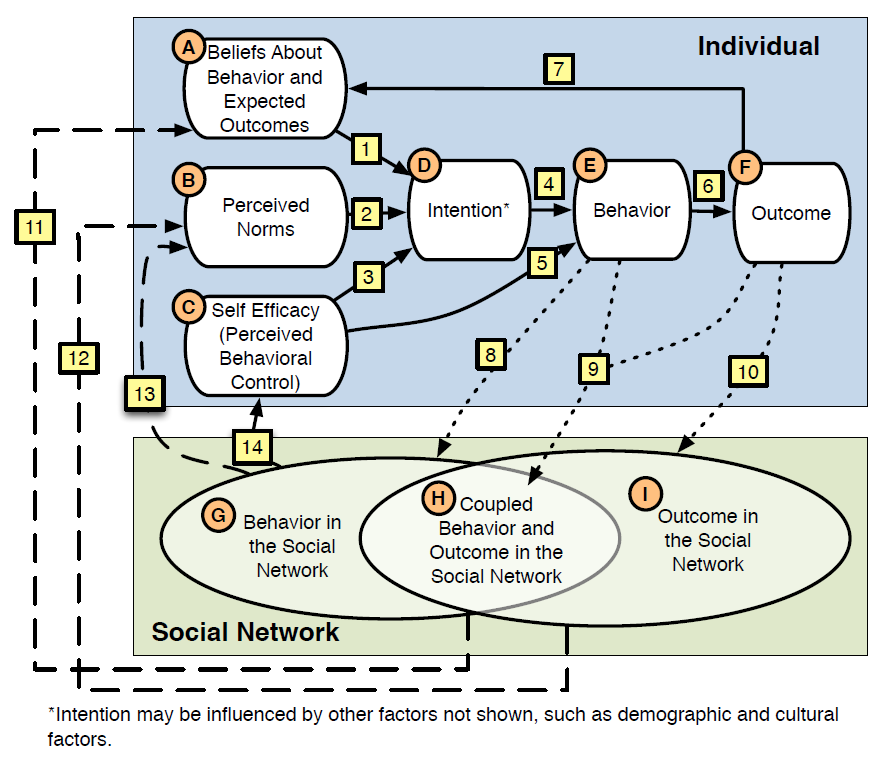
\includegraphics[width=0.7\linewidth]{figuras/influencia.png}
%%		\caption{}
%		\label{fig:influencia}
%	\end{figure}
%	
%\end{frame}

\begin{frame}
	\frametitle{Contagio social}
\begin{itemize}
	\item Los resultados globales influyen en los factores comportamentales a nivel individual, a partir de la \textit{heurística de disponibilidad} (Tversky \& Kahneman, 1974).
    \item Los modelos de contagio social describen cómo los comportamientos se transmiten a través de una población.
    \item Si algún comportamiento se convierte en más usual, tienden a percibirse como más comunes lo cual aumenta la probabilidad que otros adopten este comportamiento (instituciones económicas según Aoki).
\end{itemize}
\end{frame}

\begin{frame}
	\frametitle{Voting Model}
\begin{itemize}
	\item En \textbf{Archivo / Biblioteca de Modelos / Sample Models / IABM Textbook / "Voting Sensitivity Analysis"}
	\item Chequear:
	\begin{itemize}
		\item ¿cuántos tipos de agentes tenemos en este modelo?
		\item ¿qué variables son específicas de estos agentes? 
		\item ¿cuáles son las variables globales?
		\item ¿qué procedimientos hay en este modelo?
	\end{itemize}
\end{itemize}		
\end{frame}

\begin{frame}
	\frametitle{Voting Model}
\framesubtitle{Modificaciones}
\begin{enumerate}
	\item Agregar gráficos y monitores para visualizar la proporción de cada tipo.
	\item Suponer que en cada momento, una proporción $\alpha=5\%$ decide su voto de forma aleatoria.
	\item Asumir que los individuos tienen información pasada sobre el resultado de las elecciones (o encuestas) y esto repercute marginalmente, sólo en caso de desempate en la variable \textbf{total}. ¿Cambian drásticamente los resultados?
	\item Suponer que no todos los individuos en este mundo simulado tienen el mismo grado de influencia.
	\begin{itemize}
		\item En el caso habitual, todos tienen un `` grado de influencia'' igual a 1. En este caso, la influencia será un valor aleatorio entre [ 1 - $\gamma$ , 1 + $\gamma$]. 
	\end{itemize}  
	\item Partiendo de una distribución aleatoria de los votantes en el espacio y en sus proporciones iniciales, ¿bajo qué condiciones podemos alcanzar consensos?  
\end{enumerate}
\end{frame}

\begin{frame}
\frametitle{Otros ejemplos: preferencias sociales}
The utility function of these agents can be written as: 
\begin{equation}
u_{i,t}(c,\tau, m) = \frac{a}{C}*f_i(c) + b*m_{c,t} - d*m_{c',t}
\end{equation} 
where:
\begin{itemize}
\small	\item $ f(c)$ are individual preferences, exogenous to the model, with $ f(c) > 0 $ if $ c = \tau $ (preferred crowding type) and $ f(c) = 0 $ in other cases.
	\item $m_{c,t}$ is the proportion of agents with crowding type $c$ in the period $ t $ and $m_{c',t}$ is equal to the proportion of agents with a crowding type other than $ c $ in $ t $, \textit{in the neighborhood of i}.
	\item $C$ is the number of crowding types available.
	\item $a$, $b$ and $d$ are the parameters that will allow us to study other behaviors from the base-configuration, with $ a = b = d = 1 $
\end{itemize}
\end{frame}

\begin{frame}
	\frametitle{Otros ejemplos: confianza en los Bancos Centrales y tolerancia a los desvíos}
\begin{itemize}
\small	\item Central Bank's credibility ($\chi_{it}$, Eq. \eqref{eq3}) determines whether agents in the next period will be based mostly on the target or trend inflation (Eq. \eqref{eq4}).
	\item It is measured each period; w¸e assume $\chi^{min}_{it} = 0.1 $ and $\chi^{max}_{it}=0.9$, with $\Delta_{i}$ as tolerance to the Central Bank. 
\end{itemize} 

\begin{equation}
\chi_{it}= 1-\dfrac{|\pi^T_t-\pi_t|}{\Delta_{i}}\text{ , with } \Delta_{i}\sim U[0,\delta]
\label{eq3}
\end{equation}

\begin{itemize}
\small	\item Credibility is time-dependent; this implies that Central Bank's credibility arises from their performance.
	\item  Parameter $\Delta_{i}$, defined as individual tolerance to the Central Bank policy, is an indirect measure of the maximum deviation from the target so that the target is no longer credible.
\end{itemize} 

\begin{equation}
\pi^e_{i,t+1} = \pi^T_{it} \chi_{it} + \pi^{trend}_{it} (1 - \chi_{it})
\label{eq4}
\end{equation}	
\end{frame}

\begin{frame}
\frametitle{Modeling Commons}
\begin{itemize}
	\item Sitio web creado para compartir y discutir Modelos Basados en Agentes escritos en Netlogo.
	\item Más de 2500 modelos de diferentes disciplinas.
	\item Posibilidad de crear, compartir y comentar modelos.
	\item Accesible a través de \url{http://modelingcommons.org/}
\end{itemize}
\end{frame}


\begin{frame}
	\frametitle{Modeling Commons}
	\framesubtitle{ejemplo: COVID}
Modelo: \textit{\textbf{Disease, Social Distancing, Economic Impact }}
	\begin{itemize}
		\item Ingresar a \url{http://modelingcommons.org/browse/one_model/6264}
		\item observar en la web:
		\begin{itemize}
			\item ¿qué información sobre el modelo se encuentra disponible?
			\item ¿podemos correr el modelo desde la web?
			\item ¿qué ventajas y desventajas tiene Modeling Commons?
			\item ¿hay otros modelos que surgen de éste? ¿qué extensiones ofrecen?		
\item ¿en qué se diferencia de los otros modelos?
\item ¿sus supuestos son razonables?
\item ¿qué resultados ofrece este modelo?
		\end{itemize}
		\item Otros ejemplos: Modelo \textit{\textbf{COVID\_19 Spread}}
		\begin{itemize}
		\item Ingresar a \url{http://modelingcommons.org/browse/one_model/6227}
		\end{itemize}
	\end{itemize}
\end{frame}


\end{document}
